% ===========================================================================
\section{Extension: massive neutrinos}\label{sec:neutrinos}
% ===========================================================================

Neutrino oscillations show that at least two neutrino species are massive, with $\sum m_\nu\gtrsim0.06$\,eV. For
cosmology the masses matter because the neutrinos become non-relativistic in the late universe: before that they
behave like radiation, afterwards like a hot component of the dark matter that does not cluster on small scales. We
add one massive species of mass $m_\nu$ (the minimal normal-ordering case, if the lighter ones are treated as
massless), following Refs.~\cite{Ma1995,LesgourguesTram2011,LesgourguesPastor2006}. As in CLASS, its temperature
today is $T_{\nu}=0.71611\,T_{\rm CMB}$, which gives $\Om_\nu h^2=m_\nu/93.14$\,eV and contributes $1.0132$ to
$N_{\rm eff}$; the other $N_{\rm eff}-1.0132=2.0328$ species stay massless. We keep $h$, $\omega_b$ and $\omega_{\rm cdm}$
of the fiducial model, so that $\Om_\Lambda$ absorbs the neutrino density.

\subsection{Theory}

\paragraph*{Background.} The neutrinos decoupled at $T\sim1$\,MeV while relativistic, so their distribution keeps the
relativistic Fermi--Dirac form $f_0(q)=1/(e^q+1)$ in the comoving momentum $q=ap/(k_BT_{\nu})$, even after they
become non-relativistic. With $M(a)=am_\nu c^2/(k_BT_{\nu})$ the comoving energy is $\epsilon=\sqrt{q^2+M^2}$, and
\begin{align}
\rho_\nu&=\frac{15}{\pi^4}\Big(\frac{T_\nu}{T_{\rm CMB}}\Big)^4\frac{\rho_{\gamma0}}{a^4}\int_0^\infty dq\,q^2\epsilon f_0,\\
p_\nu&=\frac{15}{\pi^4}\Big(\frac{T_\nu}{T_{\rm CMB}}\Big)^4\frac{\rho_{\gamma0}}{a^4}\int_0^\infty dq\,\frac{q^4}{3\epsilon}f_0 .
\end{align}
For $M\ll1$ this is radiation ($p=\rho/3$, $\rho\propto a^{-4}$); for $M\gg1$, $\rho\to\frac{3\zeta(3)}{2}M$ times the
prefactor, i.e.\ matter with $\rho\propto a^{-3}$. The transition, $M\approx3$, happens at $1+z\approx M_0/3$, i.e.\
$z_{\rm nr}=118$, 296 and 594 for $m_\nu=0.06$, 0.15 and 0.3\,eV (Fig.~\ref{fig:nu}a). The derivatives needed for
$\mathcal H'$ and $\mathcal H''$ follow from $\rho'=-3(\rho+p)$ and $p'=-(5p-\mathfrak p)$, where
$\mathfrak p=\frac{15}{\pi^4}(\dots)\int dq\,q^6f_0/(3\epsilon^3)$ is the ``pseudo-pressure''. We evaluate the
integrals with 48-point Gauss--Laguerre quadrature, accurate to $10^{-7}$; age and conformal time agree with CLASS in
all printed digits.

\paragraph*{Perturbations.} A massive particle's velocity, $q/\epsilon$, depends on its momentum, so the perturbation
cannot be described by a single temperature multipole hierarchy. Following Ma and Bertschinger~\cite{Ma1995} we write
$f=f_0(q)[1+\Psi(\bm k,\hat n,q,\eta)]$ and expand $\Psi$ in Legendre multipoles $\Psi_\ell(q)$ for a set of momenta
$q_i$. In our variables ($\kappa=ck/\mathcal H$, Newtonian gauge),
\begin{align}
\Psi_0' &= -\kappa\frac{q}{\epsilon}\Psi_1+\Phi'\frac{d\ln f_0}{d\ln q},\\
\Psi_1' &= \frac{\kappa}{3}\frac{q}{\epsilon}\big(\Psi_0-2\Psi_2\big)-\frac{\kappa}{3}\frac{\epsilon}{q}\Psi\frac{d\ln f_0}{d\ln q},\\
\Psi_\ell' &= \frac{\kappa}{2\ell+1}\frac{q}{\epsilon}\big[\ell\Psi_{\ell-1}-(\ell+1)\Psi_{\ell+1}\big],\quad \ell\ge2 .
\end{align}
The free-streaming terms are those of massless neutrinos with $c$ replaced by the particle velocity $cq/\epsilon$,
and the metric terms act through $d\ln f_0/d\ln q$: a potential well shifts all momenta, which changes $f$ in
proportion to its slope. The neutrinos enter the Einstein equations through their density, velocity and shear,
\begin{align}
\delta\rho_\nu&\propto\int dq\,q^2\epsilon f_0\Psi_0,\nonumber\\
(\rho+p)_\nu\theta_\nu&\propto k\int dq\,q^3f_0\Psi_1,\nonumber\\
(\rho+p)_\nu\sigma_\nu&\propto\frac23\int dq\,\frac{q^4}{\epsilon}f_0\Psi_2,
\end{align}
which replace $4\rho_\nu\mathcal N_0$ and the shear of $\mathcal N_2$ in Eqs.~\eqref{eq:einstein1}--\eqref{eq:einstein2}. For
$M\to0$ and $\Psi_\ell=-\mathcal N_\ell\,d\ln f_0/d\ln q$ the system reduces exactly to the massless one, which also
gives the adiabatic initial conditions. We use 8 Gauss--Laguerre momenta and $\ell_{\max}=17$ (as CLASS); 16 momenta
or $\ell_{\max}=25$ change $C_\ell$ and $P(k)$ by less than $3\times10^{-5}$.

\paragraph*{Fluid approximation.} Deep inside the horizon ($k\eta>31$) the hierarchy is replaced by the fluid
equations of Ref.~\cite{LesgourguesTram2011} for $\delta_\nu$, $\theta_\nu$ and $\sigma_\nu$, with the adiabatic sound
speed $c_a^2=\frac{w}{3(1+w)}(5-\mathfrak p/p)$ and a viscosity closure for the shear, as in CLASS. This reduces the
system from 190 to 49 variables. Compared with the full hierarchy it changes $P(k)$ by up to 0.3\% at
$m_\nu=0.3$\,eV; CLASS's fluid approximation has the same error, to $10^{-4}$. With 190 variables the
dense linear algebra of the implicit (BDF) solver makes it about 20 times slower than an explicit Runge--Kutta
method, which gives identical results while the hierarchy is active; we use the explicit method there. A run with
massive neutrinos then takes 40--43\,s for the perturbations on 2 cores, compared with 37\,s for massless neutrinos.

\paragraph*{Matter power spectrum.} With massive neutrinos the total matter is CDM, baryons and neutrinos. We compute
the comoving density contrast directly,
$\Delta_m=\sum_i\rho_i[\delta_i-3(1+w_i)\mathcal Hv_i/(ck)]/\sum_i\rho_i$, which is the synchronous-gauge $\delta_m$
used by CLASS; for massless neutrinos it agrees with the Poisson equation~\eqref{eq:DeltaM} up to radiation terms of
order $10^{-3}$ at $k\sim10^{-4}\Mpc^{-1}$, and reduces the difference from CLASS there from $2\times10^{-3}$ to
$10^{-5}$. We also output the CDM+baryon spectrum $P_{cb}$, the relevant one for galaxy clustering.

\begin{figure*}
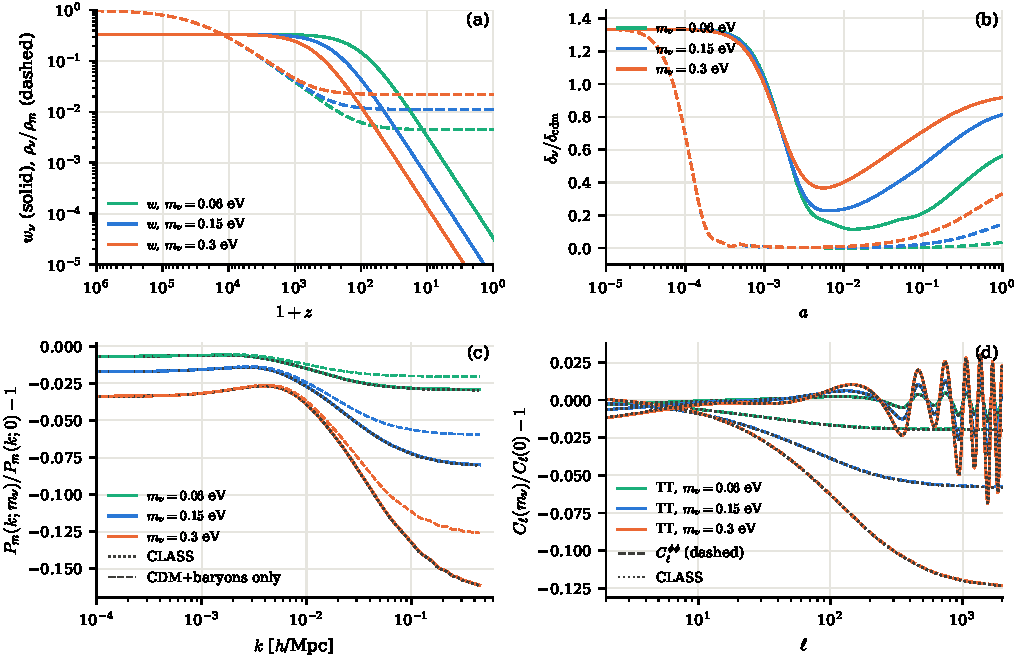
\includegraphics[width=0.95\textwidth]{neutrinos}
\caption{Massive neutrinos with $m_\nu=0.06$, 0.15 and 0.3\,eV (fixed $h$, $\omega_b$, $\omega_{\rm cdm}$).
\emph{(a)} Equation of state $w_\nu$ and density relative to all matter. \emph{(b)} $\delta_\nu/\delta_{\rm cdm}$ for
$k=0.01\Mpc^{-1}$ (solid) and $0.1\Mpc^{-1}$ (dashed): below the free-streaming scale the neutrinos stop clustering, and fall back into the CDM wells after they
slow down. \emph{(c)} Change of the total matter power spectrum (solid) and of the CDM+baryon spectrum (dashed)
today, with CLASS (dotted). \emph{(d)} Change of the unlensed TT spectrum (solid) and the lensing potential (dashed),
with CLASS (dotted).}
\label{fig:nu}
\end{figure*}

\subsection{Results}

\paragraph*{Free streaming.} While relativistic, neutrinos stream out of any structure smaller than the horizon.
After $z_{\rm nr}$ their thermal velocity $\langle v\rangle\approx3.15\,k_BT_\nu/(m_\nu a)$ decays, and the
free-streaming scale, the distance travelled in a Hubble time, shrinks. Its comoving wavenumber
$k_{\rm fs}\sim\sqrt{3/2}\,\mathcal H/\langle v\rangle$ grows as $a^{1/2}$ in matter domination; the smallest value
reached, at $z_{\rm nr}$, is $k_{\rm nr}\approx0.018\sqrt{\Om_m m_\nu/{\rm eV}}\,h\Mpc^{-1}\approx0.003$--$0.006\,h\Mpc^{-1}$.
Figure~\ref{fig:nu}b shows the consequence. Initially $\delta_\nu=\frac43\delta_{\rm cdm}$ (adiabatic). When a mode
enters the horizon the neutrino perturbation decays by free streaming. Later, when $k<k_{\rm fs}(a)$, the neutrinos
fall into the CDM potential wells and $\delta_\nu\to\delta_{\rm cdm}$: at $k=0.01\Mpc^{-1}$ this has largely happened
today for 0.3\,eV, but at $k=0.1\Mpc^{-1}$ the neutrinos still lag far behind.

\paragraph*{Matter power spectrum.} On scales above $k_{\rm nr}$ neutrinos behave like CDM, and $P(k)$ changes only
by $0.6$--3\% because $\Om_\Lambda$ is smaller (Fig.~\ref{fig:nu}c). Below the free-streaming scale the spectrum is
suppressed, by $2.9\%$, $8.0\%$ and $16.1\%$ at $k=0.5\,h\Mpc^{-1}$ for the three masses (CLASS: 3.0, 8.0, 16.2\%).
There are two reasons~\cite{HuEisensteinTegmark1998,LesgourguesPastor2006}. First, a fraction
$f_\nu=\Om_\nu/\Om_m=0.0045$, 0.011, 0.022 of the matter does not cluster, which removes $2f_\nu$ from
$P_m\propto[(1-f_\nu)\delta_{cb}]^2$. Second, the CDM and baryons grow more slowly, since only a fraction $1-f_\nu$ of
the matter falls into the wells: $\delta_{cb}\propto a^{1-3f_\nu/5}$ instead of $a$, which accumulates to a
suppression of $P_{cb}$ of several $f_\nu$. Together the suppression is $\approx-8f_\nu$ asymptotically; at
$k=0.5\,h\Mpc^{-1}$ we find $-6.5f_\nu$, $-7.1f_\nu$ and $-7.3f_\nu$. The CDM+baryon spectrum shows only the second
effect. This step-like suppression is why galaxy surveys are sensitive to $\sum m_\nu$.

\paragraph*{CMB.} The masses we consider make the neutrinos non-relativistic well after recombination, so the
primary anisotropies change only through the background. The extra matter today shortens the distance to the
last-scattering surface ($\eta_0$ decreases by 118\,Mpc for 0.3\,eV), which moves the peaks to lower $\ell$ (the
first from 221 to 219) and causes the oscillating residuals in Fig.~\ref{fig:nu}d. The lower $\Om_\Lambda$ reduces
the late ISW effect, and for 0.3\,eV the neutrinos are no longer fully relativistic at decoupling, which changes the
early ISW effect. The lensing potential, a projection of the matter distribution, is suppressed like $P(k)$: at
$\ell=1000$ by 1.9\%, 5.7\% and 12.0\%. CMB lensing therefore constrains the neutrino mass: through the smoothing of the peaks
(Sec.~\ref{sec:lensing}) and through direct reconstructions of $C_\ell^{\phi\phi}$.

\paragraph*{Validation.} We compare the effect of the mass, $X(m_\nu)/X(0)-1$, with CLASS run with the same
parameters (which removes the recombination differences of Sec.~\ref{sec:validation}). For $m_\nu=0.06$\,eV, the
effects on TT, lensed TT, $C_\ell^{\phi\phi}$ and $P_m$ agree to $3$--$5\times10^{-4}$ and on EE to $6\times10^{-4}$;
for 0.3\,eV to $8\times10^{-4}$, $1.0\times10^{-3}$, $3\times10^{-4}$, $4\times10^{-4}$ and $3.7\times10^{-3}$, i.e.\
better than 3\% of the effect itself. A nearly massless species ($m_\nu=10^{-4}$\,eV) reproduces the massless
neutrinos to $4\times10^{-7}$ in $\Phi$ at recombination when the same $\ell_{\max}$ is used.
